
\documentclass[11pt]{article}
\usepackage[a4paper,margin=1in]{geometry}
\usepackage{amsmath,amssymb}
\usepackage{graphicx}
\usepackage[dvipsnames]{xcolor}
\usepackage{hyperref}
\usepackage{enumitem}
\usepackage{tabularx}
\usepackage{longtable}
\usepackage{booktabs}
\usepackage[most]{tcolorbox}
\usepackage{titlesec}
\usepackage{xurl}
\usepackage{fancyhdr}
\usepackage{setspace}
\usepackage{tikz}
\usetikzlibrary{positioning,arrows.meta}
\usepackage[T1]{fontenc}
\usepackage{lmodern}
\setlength{\parindent}{0pt}
\setlength{\parskip}{8pt}
\setlength{\headheight}{14pt}
\setstretch{1.12}
\setlist[itemize]{leftmargin=1.5em, nosep}
\setlist[enumerate]{leftmargin=1.5em, nosep}
\providecommand{\tightlist}{\setlength{\itemsep}{0pt}\setlength{\parskip}{0pt}}
\hypersetup{colorlinks=true,linkcolor=MidnightBlue,urlcolor=MidnightBlue}
\pagestyle{fancy}
\fancyhf{}
\rhead{\thepage}
\renewcommand{\headrulewidth}{0pt}
\renewcommand{\footrulewidth}{0pt}
\titleformat{\section}{\Large\bfseries\color{MidnightBlue}}{\thesection}{0.6em}{}
\titleformat{\subsection}{\bfseries}{}{0em}{}


\begin{document}

\begin{center}\LARGE\bfseries Exact Inference in Bayesian Networks\end{center}

\begin{center}\large Block 4 Day 2\end{center}

\begin{tcolorbox}[colback=MidnightBlue!4,colframe=MidnightBlue,title={Session Overview},fonttitle=\bfseries,breakable]
\textbf{Session objective:} Strengthen exact inference through worked enumeration, elimination-order reasoning, and complexity awareness without copying likely exam arithmetic exactly.

\textbf{Timing target (min):} 71

\textbf{Topic anchors:} exact inference; enumeration; variable elimination; elimination order; treewidth

\textbf{Padlet board:} \url{https://padlet.com/qmul/b4-d2-cxmnkit5wkn83isk}
\end{tcolorbox}

\section*{Exercises}

\begin{tcolorbox}[colback=white,colframe=MidnightBlue,title={Q1 Core Concept Check},fonttitle=\bfseries,breakable]
\begin{center}
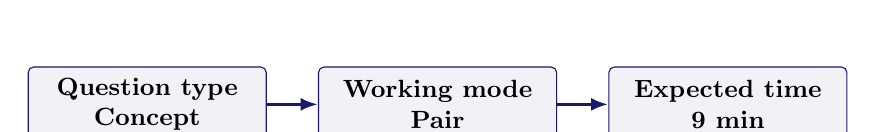
\begin{tikzpicture}[
node distance=0.65cm,
box/.style={draw=MidnightBlue, rounded corners=2pt, minimum height=0.95cm, align=center, font=\small\bfseries, fill=MidnightBlue!6, text width=0.23\linewidth},
arrow/.style={-{Latex[length=2.2mm]}, very thick, MidnightBlue}
]
\node[box] (type) {Question type\\Concept};
\node[box, right=of type] (mode) {Working mode\\Pair};
\node[box, right=of mode] (time) {Expected time\\9 min};
\draw[arrow] (type) -- (mode);
\draw[arrow] (mode) -- (time);
\end{tikzpicture}
\end{center}

{\large\bfseries\color{MidnightBlue} Prompt}\par\medskip
Contrast exact and approximate inference using three ideas: guarantee of the answer, computational cost, and when each approach is preferable in a live system.

{\large\bfseries\color{MidnightBlue} Task details}\par\medskip
\begin{itemize}\item \textbf{Type:} concept
\item \textbf{Mode:} pair
\item \textbf{Time:} 9 min
\item \textbf{Deliverable:} comparison table
\item \textbf{Assessment focus:} contrast exact and approximate inference in practical terms
\item \textbf{Expected length:} 3 rows\end{itemize}

{\large\bfseries\color{MidnightBlue} How to submit}\par\medskip
Post one pair Padlet comment as a three-row comparison table or numbered list.

{\large\bfseries\color{MidnightBlue} Discussion in class}\par\medskip
Why do teams still use exact inference if it can become expensive?

{\large\bfseries\color{MidnightBlue} Why this helps}\par\medskip
Useful for short comparison questions before the mathematical work begins.

{\large\bfseries\color{MidnightBlue} References}\par\medskip
\begin{itemize}\item Russell \& Norvig (2021) AIMA 4e, Ch.13, pp.412-460
\item Poole \& Mackworth (2023) 3e, Ch.9, pp.375-458\end{itemize}
\end{tcolorbox}

\begin{tcolorbox}[colback=white,colframe=MidnightBlue,title={Q2 Structured Problem},fonttitle=\bfseries,breakable]
\begin{center}
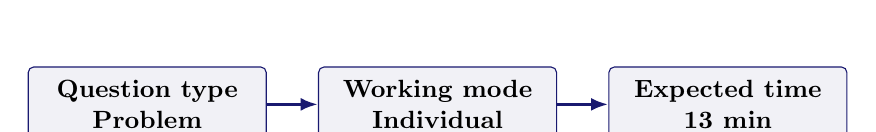
\begin{tikzpicture}[
node distance=0.65cm,
box/.style={draw=MidnightBlue, rounded corners=2pt, minimum height=0.95cm, align=center, font=\small\bfseries, fill=MidnightBlue!6, text width=0.23\linewidth},
arrow/.style={-{Latex[length=2.2mm]}, very thick, MidnightBlue}
]
\node[box] (type) {Question type\\Problem};
\node[box, right=of type] (mode) {Working mode\\Individual};
\node[box, right=of mode] (time) {Expected time\\13 min};
\draw[arrow] (type) -- (mode);
\draw[arrow] (mode) -- (time);
\end{tikzpicture}
\end{center}

{\large\bfseries\color{MidnightBlue} Prompt}\par\medskip
Use the Alarm network numbers from class: P(B)=0.001, P(E)=0.002, P(A\textbar B,E)=0.95, P(A\textbar B,\textasciitilde E)=0.94, P(A\textbar\textasciitilde B,E)=0.29, P(A\textbar{}\textsubscript{B,}E)=0.001, P(J\textbar A)=0.90, P(J\textbar\textasciitilde A)=0.05, P(M\textbar A)=0.70, P(M\textbar\textasciitilde A)=0.01. Compute P(E=true \textbar{} J=true, M=false) by enumeration, including normalization.

\begin{tcolorbox}[colback=ForestGreen!5,colframe=ForestGreen,title={Formula reminder},fonttitle=\bfseries,breakable]
\[
P(X \mid e)=\alpha \, P(X,e)
\]
\[
P(X,e)=\sum_{h} P(X,e,h)
\]
\textbf{Use this when you must compute two unnormalised scores and then normalise.}
\end{tcolorbox}

{\large\bfseries\color{MidnightBlue} Task details}\par\medskip
\begin{itemize}\item \textbf{Type:} problem
\item \textbf{Mode:} individual
\item \textbf{Time:} 13 min
\item \textbf{Deliverable:} worked enumeration
\item \textbf{Assessment focus:} carry out one exact inference query by enumeration with normalization
\item \textbf{Expected length:} 5 calculation lines\end{itemize}

{\large\bfseries\color{MidnightBlue} How to submit}\par\medskip
Post your own Padlet comment showing the two unnormalized scores, the normalization step, and the final probability.

{\large\bfseries\color{MidnightBlue} Discussion in class}\par\medskip
Which hidden variables do you need to sum out, and why?

{\large\bfseries\color{MidnightBlue} Why this helps}\par\medskip
Direct practice for exact enumeration while using a different target query from the exam set.

{\large\bfseries\color{MidnightBlue} References}\par\medskip
\begin{itemize}\item Russell \& Norvig (2021) AIMA 4e, Ch.13, pp.412-460
\item Poole \& Mackworth (2023) 3e, Ch.9, pp.375-458\end{itemize}
\end{tcolorbox}

\begin{tcolorbox}[colback=white,colframe=MidnightBlue,title={Q3 Structured Problem},fonttitle=\bfseries,breakable]
\begin{center}
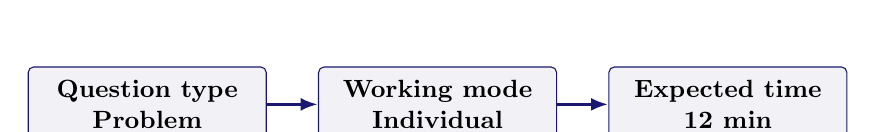
\begin{tikzpicture}[
node distance=0.65cm,
box/.style={draw=MidnightBlue, rounded corners=2pt, minimum height=0.95cm, align=center, font=\small\bfseries, fill=MidnightBlue!6, text width=0.23\linewidth},
arrow/.style={-{Latex[length=2.2mm]}, very thick, MidnightBlue}
]
\node[box] (type) {Question type\\Problem};
\node[box, right=of type] (mode) {Working mode\\Individual};
\node[box, right=of mode] (time) {Expected time\\12 min};
\draw[arrow] (type) -- (mode);
\draw[arrow] (mode) -- (time);
\end{tikzpicture}
\end{center}

{\large\bfseries\color{MidnightBlue} Prompt}\par\medskip
Consider a network with edges Season -\textgreater{} Pollen, Season -\textgreater{} Flu, Pollen -\textgreater{} Sneezing, Flu -\textgreater{} Fever, Flu -\textgreater{} Sneezing. For the query P(Flu \textbar{} Sneezing=true), choose an elimination order for Season, Pollen, and Fever, and explain briefly what factor would become awkward if you eliminated the wrong variable too early.

{\large\bfseries\color{MidnightBlue} Task details}\par\medskip
\begin{itemize}\item \textbf{Type:} problem
\item \textbf{Mode:} individual
\item \textbf{Time:} 12 min
\item \textbf{Deliverable:} elimination trace
\item \textbf{Assessment focus:} reason about factor growth under variable elimination
\item \textbf{Expected length:} ordered list + 3 short notes\end{itemize}

{\large\bfseries\color{MidnightBlue} How to submit}\par\medskip
Post your own Padlet comment with the order and three short notes on factor growth.

{\large\bfseries\color{MidnightBlue} Discussion in class}\par\medskip
Which hidden variable acts like the most dangerous hub in this network?

{\large\bfseries\color{MidnightBlue} Why this helps}\par\medskip
Useful for variable-elimination reasoning without copying the exact financial-risk exam scenario.

{\large\bfseries\color{MidnightBlue} References}\par\medskip
\begin{itemize}\item Russell \& Norvig (2021) AIMA 4e, Ch.13, pp.412-460
\item Poole \& Mackworth (2023) 3e, Ch.9, pp.375-458\end{itemize}
\end{tcolorbox}

\begin{tcolorbox}[colback=white,colframe=MidnightBlue,title={Q4 Collaborative Mini-Case},fonttitle=\bfseries,breakable]
\begin{center}
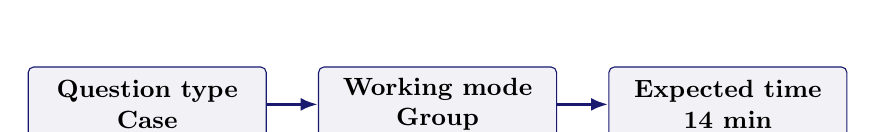
\begin{tikzpicture}[
node distance=0.65cm,
box/.style={draw=MidnightBlue, rounded corners=2pt, minimum height=0.95cm, align=center, font=\small\bfseries, fill=MidnightBlue!6, text width=0.23\linewidth},
arrow/.style={-{Latex[length=2.2mm]}, very thick, MidnightBlue}
]
\node[box] (type) {Question type\\Case};
\node[box, right=of type] (mode) {Working mode\\Group};
\node[box, right=of mode] (time) {Expected time\\14 min};
\draw[arrow] (type) -- (mode);
\draw[arrow] (mode) -- (time);
\end{tikzpicture}
\end{center}

{\large\bfseries\color{MidnightBlue} Prompt}\par\medskip
You are comparing two Bayesian networks for a live monitoring system. Network A is sparse and tree-like. Network B has many cross-links between risk variables. Write a short memo explaining which one is safer for exact inference under latency pressure, and why.

{\large\bfseries\color{MidnightBlue} Task details}\par\medskip
\begin{itemize}\item \textbf{Type:} case
\item \textbf{Mode:} group
\item \textbf{Time:} 14 min
\item \textbf{Deliverable:} complexity memo
\item \textbf{Assessment focus:} explain why one network is easier than another for exact inference
\item \textbf{Expected length:} 4 bullets\end{itemize}

{\large\bfseries\color{MidnightBlue} How to submit}\par\medskip
Post one group Padlet comment with four bullets and one recommended operational choice.

{\large\bfseries\color{MidnightBlue} Discussion in class}\par\medskip
Is graph size or graph shape the more dangerous issue for exact inference?

{\large\bfseries\color{MidnightBlue} Why this helps}\par\medskip
Supports exam-style complexity reasoning without turning the prompt into a definition-only question.

{\large\bfseries\color{MidnightBlue} References}\par\medskip
\begin{itemize}\item Russell \& Norvig (2021) AIMA 4e, Ch.13, pp.412-460
\item Poole \& Mackworth (2023) 3e, Ch.9, pp.375-458\end{itemize}
\end{tcolorbox}

\begin{tcolorbox}[colback=white,colframe=MidnightBlue,title={Q5 Exam-Style Constructed Response},fonttitle=\bfseries,breakable]
\begin{center}
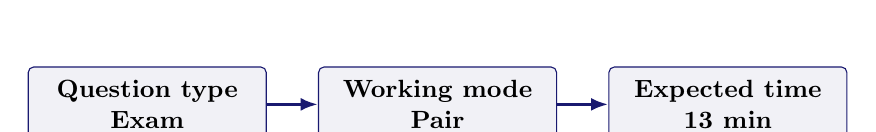
\begin{tikzpicture}[
node distance=0.65cm,
box/.style={draw=MidnightBlue, rounded corners=2pt, minimum height=0.95cm, align=center, font=\small\bfseries, fill=MidnightBlue!6, text width=0.23\linewidth},
arrow/.style={-{Latex[length=2.2mm]}, very thick, MidnightBlue}
]
\node[box] (type) {Question type\\Exam};
\node[box, right=of type] (mode) {Working mode\\Pair};
\node[box, right=of mode] (time) {Expected time\\13 min};
\draw[arrow] (type) -- (mode);
\draw[arrow] (mode) -- (time);
\end{tikzpicture}
\end{center}

{\large\bfseries\color{MidnightBlue} Prompt}\par\medskip
Explain treewidth in simple language to an engineering manager who only cares about runtime. Then explain one practical thing the team can do when exact inference becomes too costly.

{\large\bfseries\color{MidnightBlue} Task details}\par\medskip
\begin{itemize}\item \textbf{Type:} exam
\item \textbf{Mode:} pair
\item \textbf{Time:} 13 min
\item \textbf{Deliverable:} written analysis
\item \textbf{Assessment focus:} explain treewidth and one mitigation in plain language
\item \textbf{Expected length:} 180-230 words\end{itemize}

{\large\bfseries\color{MidnightBlue} How to submit}\par\medskip
Post one pair Padlet comment with a plain-language explanation, one operational consequence, and one mitigation.

{\large\bfseries\color{MidnightBlue} Discussion in class}\par\medskip
Is switching to approximate inference the only sensible mitigation?

{\large\bfseries\color{MidnightBlue} Why this helps}\par\medskip
Matches exam-style complexity explanation, but the audience and framing are different from the paper question.

{\large\bfseries\color{MidnightBlue} References}\par\medskip
\begin{itemize}\item Russell \& Norvig (2021) AIMA 4e, Ch.13, pp.412-460
\item Poole \& Mackworth (2023) 3e, Ch.9, pp.375-458\end{itemize}
\end{tcolorbox}

\begin{tcolorbox}[colback=white,colframe=MidnightBlue,title={Q6 Stretch Extension},fonttitle=\bfseries,breakable]
\begin{center}
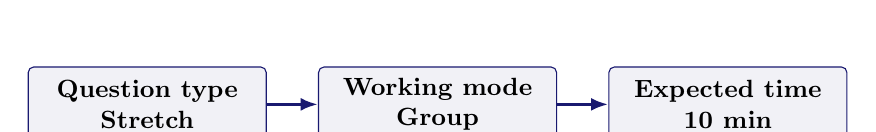
\begin{tikzpicture}[
node distance=0.65cm,
box/.style={draw=MidnightBlue, rounded corners=2pt, minimum height=0.95cm, align=center, font=\small\bfseries, fill=MidnightBlue!6, text width=0.23\linewidth},
arrow/.style={-{Latex[length=2.2mm]}, very thick, MidnightBlue}
]
\node[box] (type) {Question type\\Stretch};
\node[box, right=of type] (mode) {Working mode\\Group};
\node[box, right=of mode] (time) {Expected time\\10 min};
\draw[arrow] (type) -- (mode);
\draw[arrow] (mode) -- (time);
\end{tikzpicture}
\end{center}

{\large\bfseries\color{MidnightBlue} Prompt}\par\medskip
A fraud-monitoring system must respond within 300 milliseconds. Write a short fallback policy saying when the system should stop using exact inference, what it should use instead, and how the team should monitor that fallback.

{\large\bfseries\color{MidnightBlue} Task details}\par\medskip
\begin{itemize}\item \textbf{Type:} stretch
\item \textbf{Mode:} group
\item \textbf{Time:} 10 min
\item \textbf{Deliverable:} fallback policy
\item \textbf{Assessment focus:} define an operational switch from exact to approximate inference
\item \textbf{Expected length:} 4 policy rules\end{itemize}

{\large\bfseries\color{MidnightBlue} How to submit}\par\medskip
Post one group Padlet comment with a threshold, a fallback method class, and one monitoring rule.

{\large\bfseries\color{MidnightBlue} Discussion in class}\par\medskip
What signal should trigger the switch first: latency, memory use, or factor size warning?

{\large\bfseries\color{MidnightBlue} Why this helps}\par\medskip
Good extension for deployment questions that connect inference choice to live operational constraints.

{\large\bfseries\color{MidnightBlue} References}\par\medskip
\begin{itemize}\item Russell \& Norvig (2021) AIMA 4e, Ch.13, pp.412-460
\item Poole \& Mackworth (2023) 3e, Ch.9, pp.375-458\end{itemize}
\end{tcolorbox}

\section*{Submission Instructions}

Use the seeded Padlet posts for Q1--Q6. Q2 and Q3 are individual. Q1 and Q5 are pair tasks. Q4 and Q6 should be one joint group comment. Start each comment with your names or group label.

\section*{Whole-Class Debrief Prompts}

\begin{itemize}
\tightlist
\item
  Which step of enumeration created the most repeated work?
\item
  Why is elimination order a design decision rather than a purely mechanical one?
\item
  When should a real system stop insisting on exact inference?
\end{itemize}

\section*{Exam Transfer Note (Day-Level)}

Maps to exam questions on enumeration, elimination order, factor growth, treewidth, and exact-inference trade-offs.

\end{document}
